\chapter{Linguaggi, macchine astratte, teoria della computabilità}

\subsubsection{Alcune definizioni}
\begin{itemize}
    \item \textbf{Algoritmo}: sequenza \textit{finita} di istruzioni che risolve in un \textit{tempo finito} una classe di problemi
    \item \textbf{Codifica}: descrizione dell'algoritmo tramite un \textit{insieme ordinato di frasi} di un linguaggio di programmazione, che specificano le \textit{azioni} da svolgere
    \item \textbf{Programma}: testo scritto in accordo alla \textit{sintassi} e alla \textit{semantica} di un linguaggio di programmazione
\end{itemize}

\subsection{Esecuzione}
Un algoritmo esprime la soluzione a un problema, il programma è la formulazione testuale rigorosa in un dato linguaggio; l'esecuzione \textit{ordinata} delle azioni specificate porta a ottenere la soluzione da un insieme di dati in ingresso.

Viene assunta l'esistenza di un \textbf{automa esecutore}, una macchina astratta capace di eseguire le azioni dell'algoritmo.

\begin{figure}[H]
    \centering
    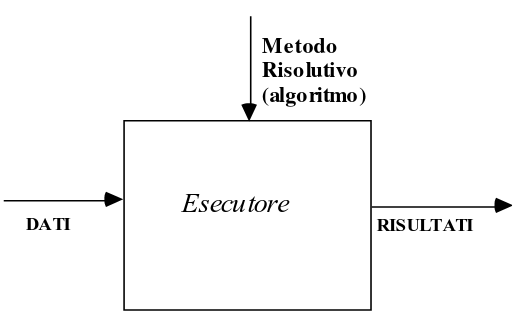
\includegraphics[width=0.6\textwidth]{/home/riccardoob/appunti/linguaggi/images/26.png}
\end{figure}

\section{Macchine astratte}

\subsection{Automa esecutore}
Un automa deve poter ricevere dall'esterno una \textit{descrizione} dell'algoritmo, deve quindi essere in grado di \textit{interpretare} un linguaggio, che verrà chiamato \textbf{linguaggio macchina}.

\subsubsection{Realizzabilità fisica}
\begin{itemize}
    \item le parti che compongono l'automa devono essere in \textit{numero finito}
    \item ingresso e uscita devono essere denotabili da un \textit{insieme finito} di \textbf{simboli}
\end{itemize}

\subsection{Gerarchia di macchine astratte}
\begin{itemize}
    \item macchina combinatoria
    \item automi a stati finiti
    \item ....
    \item macchina di Turing
\end{itemize}

Si individua una gerarchia perché diverse classi di macchina hanno diversa \textit{capacità} di risolvere problemi. Se neanche la macchina più "potente" può risolvere un problema, questo potrebbe essere \textbf{non risolubile}.

\subsection{Macchina base}
La macchina base è definita formalmente dalla tripla:
\begin{equation*}
    \langle I, O, mfn\rangle
\end{equation*}
dove
\begin{itemize}
    \item $I$ = insieme finito dei simboli di \textit{ingresso}
    \item $O$ = insieme finito dei simboli di \textit{uscita}
    \item $mfn: I \rightarrow O$ = funzione di macchina
\end{itemize}

\subsubsection{Limiti}
Utilizzare una di queste macchine per risolvere problemi comporta valutare tutte le possibili configurazioni di ingresso.

Esiste inoltre un altro limite, essendo puramente combinatoria, la macchina base non può risolvere problemi che richiedano di ricordare qualcosa dal passato, in quanto privo di memoria interna.

\subsection{Automa a stati finiti}
Nell'automa a stati finiti si introduce il concetto di memoria attraverso l'utilizzo di un numero \textit{finito} di \textbf{stati interni}.

Un \textbf{automa a stati finiti} è definito dalla quintupla:
\begin{equation*}
    \langle I, O, S, mfn, sfn\rangle
\end{equation*}
dove
\begin{itemize}
    \item $I$ = insieme finito dei simboli di \textit{ingresso}
    \item $O$ = insieme finito dei simboli di \textit{uscita}
    \item $mfn: I \times S \rightarrow O$ = funzione di macchina
    \item $sfn: I \times S \rightarrow S$ = funzione di \textbf{stato}
\end{itemize}

\subsubsection{Limiti}
Dato che lo stato funge da memoria interna, le risposte possono essere diverse a parità di dati d'ingresso.

Esistono varie categorie ASF come automi di Mealy o Moore, sincroni o asincroni, minimo numero di stati etc..

Esiste un limite computazionale che rende l'automa inadatto a risolvere problemi che non permette di limitare a priori la lunghezza delle sequenze, dovuto al fatto che la memoria è \textbf{finita}.

\subsection{Macchina di Turing}
Per ovviare al limite della memoria finita, si introduce un \textit{nastro} di memoria esterno, la \textbf{macchina di Turing} è definita dalla quintupla:
\begin{equation*}
    \langle A, S, mfn, sfn, dfn\rangle
\end{equation*}
dove
\begin{itemize}
    \item $A$ = insieme finito dei simboli di \textit{ingresso} e \textit{uscita}
    \item $S$ = insieme finito degli \textit{stati} (tra i quali \textit{HALT})
    \item $mfn: A \times S \rightarrow A$ = funzione di macchina
    \item $sfn: A \times S \rightarrow S$ = funzione di stato
    \item $dfn: A \times S \rightarrow D$ = $\{Left, Right, None\}$, funzione di \textit{direzione}
\end{itemize}

Il deposito dei dati è rappresentato da un natro illimitatamente espandibile
\begin{figure}[H]
    \centering
    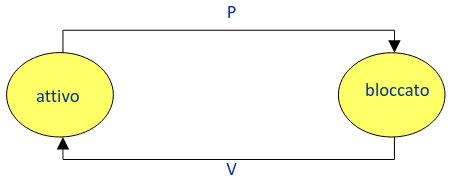
\includegraphics[width=0.8\textwidth]{/home/riccardoob/appunti/linguaggi/images/27.png}
\end{figure}

La macchina è dotata di una testina di lettura e scrittura che può:
\begin{itemize}
    \item leggere un simbolo dal nastro
    \item scrivere sul nastro il simbolo specificato da $mfn()$
    \item passare a un nuovo stato interno specificato dalla $sfn()$
    \item spostarsi sul nastro di una posizione nella direzione indicata da $dfn()$
\end{itemize}
ipotizzando che quando viene raggiunto lo stato HALT, la macchina si ferma.

Per risolvere un problema con questa macchina, è necessario definire la \textit{rappresenzatione dei dati} di partenza (da porre sul nastro) e quelli di uscita (sempre sul nastro), e definire il \textit{comportamento}, ovvero le tre funzioni $mfn()$, $sfn()$ e $dfn()$.

Non è certo che questa macchina arrivi allo stato di HALT.

\subsubsection{Tesi di Church-Turing}
Esiste una macchina più "potente" della MdT?

La tesi di Church-Turing afferma che
\begin{mdframed}[topline=false,bottomline=false,rightline=false]
    Non esiste alcun formalismo capace di risolvere una classe di problemi più ampia di quella risolta dalla macchina di Turing.
\end{mdframed}

\subsection{Macchine universali}
Nella macchina di Turing l'algoritmo è cablato nella macchina.

Si può espandere la MdT alla macchina di Turing \textbf{Universale} (UTM), macchina il cui programma è letto dalla macchina direttamente dal nastro.

Questo richiede poter descrivere l'algoritmo richiesto attraverso un \textit{linguaggio} e avere una macchina che lo interpreti.

Le tre operazioni che la UTM effettua sono:
\begin{itemize}
    \item \textbf{fetch}, ricerca delle istruzioni
    \item \textbf{decode}, interpretazione delle istruzioni
    \item \textbf{execute}, esecuzione le istruzioni
\end{itemize}

\subsubsection{UTM vs Macchina di Von Neumann}

\begin{multicols}{2}
    \noindent
    Macchina di Turing
    \begin{itemize}
        \item leggere/scrivere simbolo da/su nastro
        \item transitare in un nuovo stato
        \item spostarsi sul nastro di x posizioni
    \end{itemize}
    \columnbreak
    \begin{mdframed}[topline=false,bottomline=false,rightline=false] 
        Macchina di Von Neumann
        \begin{itemize}
            \item lettura/scrittura da/su RAM/ROM
            \item nuova configurazione registri CPU
            \item scelta cella di memoria su cui operare
        \end{itemize}
    \end{mdframed}
\end{multicols}

La UTM non ha il concetto di "mondo esterno", ne nessuna istruzione di I/O, è puramente computazione senza la dimensione di \textit{interazione}.

\subsubsection{Computazione e interazione}
Computazione e interazione sono dimensioni \textit{ortogonali}, potenzialmente espressi da due linguaggi distinti:
\begin{multicols}{2} 
    \begin{itemize}
        \item linguaggio di \textbf{computazione}
        \item linguaggio di \textbf{coordinazione}
        \begin{itemize}
            \item linguaggio di \textbf{comunicazione}
        \end{itemize}
    \end{itemize}
    \begin{mdframed}[topline=false,bottomline=false,rightline=false]
        \begin{multicolfigure}
            \centering
            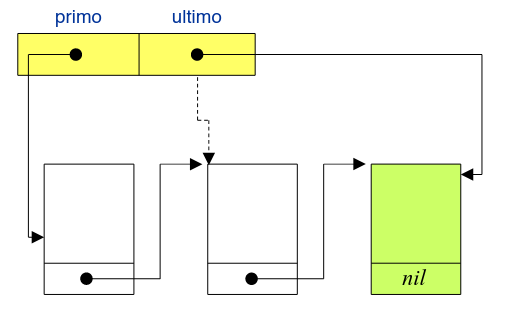
\includegraphics[width=0.6\textwidth]{/home/riccardoob/appunti/linguaggi/images/28.png}
        \end{multicolfigure}
    \end{mdframed}
\end{multicols}

\section{Teoria della computabilità}

\subsubsection{Problemi irrisolubili}
Secondo la tesi di Church-Turing, non esiste un formalismo più potente della macchina di Turing, quindi se la MdT non riesce a risolvere un problema, quel problema è \textbf{irrisolubile}.

Per irrisolubile si intende che la MdT non si ferma, quindi non ritorna un output definito.

\subsubsection{Problemi risolubili}
Un problema risolubile è un problema la cui soluzione può essere calcolata da una MdT o equivalenti.

\section{Funzioni}
Per valutare la risolubilità di un problema è necessario individuare una \textbf{funzione} che lo descrive.

\subsection{Funzione caratteristica}
Come prima cosa si definisce la funziona \textbf{caratteristica} di un problema.

\begin{mdframed}[topline=false,bottomline=false,rightline=false]
    Dato un problema $P$ e detti
    \begin{itemize}
        \item $X$ l'insieme dei suoi dati in ingresso
        \item $Y$ l'insieme delle risposte corrette
    \end{itemize}
    si dice funzione caratteristica del problema $P$
    \begin{equation*}
        f_p: X \rightarrow Y
    \end{equation*}
\end{mdframed}

In questo modo, problema non risolubile equivale a una funzione caratteristica non computabile.

\subsection{Funzione computabile}
Si formalizza ora la classe di funzioni dette \textbf{computabili}.

\begin{mdframed}[topline=false,bottomline=false,rightline=false]
    Una funzione $f:A \rightarrow B$ è detta \textit{computabile} se esiste una macchina di Turing che, data sul nastro una rappresentazione di $x \in A$, dopo un \textit{numero finito} di passi produce sul nastro una rappresentazione di $f(x) \in B$.
\end{mdframed}

\subsection{Funzioni definibili vs funzioni computabili}
É necessario capire se tutte le funzioni sono computabili, o se esistono funzioni definibili ma non computabili.

\subsubsection{Funzione computabile su N}
Per semplicità, considereremo funzioni sui \textit{numeri naturali}
\begin{equation*}
    f: N \rightarrow N
\end{equation*}
Questa condizione non è limitativa, dato che ogni informazione è necessariamente finita, può quindi essere codificata con una collezione di numeri naturali, la quale a sua volta può essere espressa tramite un \textit{unico} numero naturale (procedimento di Gödel.

\subsubsection{Procedimento di Gödel}
Data una collezione di numeri naturali, ottenere un unico numero naturale.

\begin{mdframed}[topline=false,bottomline=false,rightline=false]
    \begin{itemize}
        \item siano $N_1, N_2, \dots, N_k$ i numeri naturali dati
        \item siano $P_1, P_2, \dots, P_k$ i primi $k$ numeri primi
    \end{itemize}
    Si definisce $R$, un nuovo numero naturale così definito
    \begin{equation*}
        R ::= P_1^{N_1} \cdot P_2^{N_2} \cdot \dots \cdot P_k^{N_k}
    \end{equation*}
\end{mdframed}
R rappresenta unicamente la collezione originale $N_1, N_2, \dots, N_k$.

Poiché che l'insieme $F=\{f: N \rightarrow N\}$ delle funzioni sui naturali non è \textit{enumerabile}, e l'insieme delle funzioni computabili è enumerabile (dato che l'insieme dei simboli è finito ogni MdT può essere associata a un numero di Gödel), la gran parte delle funzioni definibili \underline{non è computabile}.

Interessano però soltanto le funzioni definibili con un linguaggio basato su un alfabeto finito di simboli, sfortunamtamento esistono funzioni definibili con tale alfabeto ma \textit{non computabili}.

\subsection{Funzioni non computabili}
Dire che esistono funzioni definibili ma non computabili, equivale a dire che esistono problemi irrisolubili, basta trovare uno solo di questi problemi.

\subsubsection{Problema dell'HALT della macchina di Turing}
\begin{mdframed}[topline=false,bottomline=false,rightline=false]
    Stabilire se una data macchina di Turing T, con un generico ingresso X, si ferma oppure no.
\end{mdframed}

Slide 49-55.

\subsection{Generabilità e decidibilità}
Poiché un linguaggio è un insieme di frasi, è utile indagare la \textbf{generabilità} e la \textbf{decidibilità} di un insieme.

Si introduce il concetto di \textit{insieme ricorsivamente numerabile}, per decidere che l'insieme sia effettivamente generabile.

\subsubsection{Insieme ricorsivamente numerabile}
Data la definizione di un insieme numerabile, ovvero un insieme i cui elementi possono essere "contati" cioè che possiede una funzione biettiva:
\begin{equation*}
    f: N \rightarrow S
\end{equation*}
che mette in corrispondenza i numeri naturali con gli elementi del sistema.

Si passa alla definizione di insieme \textbf{ricorsivamente numerabile} (\textit{semi-decidibile}). 
\begin{mdframed}[topline=false,bottomline=false,rightline=false]
    Un insieme è ricorsivamente numerabile se la funzione biettiva $f: N \rightarrow S$ è \textit{computabile}.
\end{mdframed}
\begin{figure}[H]
    \centering
    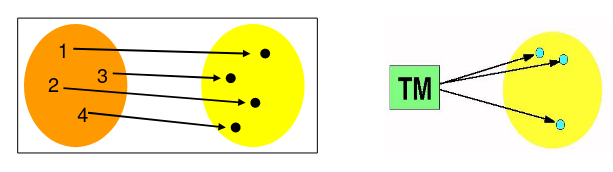
\includegraphics[width=0.6\textwidth]{/home/riccardoob/appunti/linguaggi/images/29.png}
\end{figure}
Tuttavia, il fatto che l'insieme possa essere costruito, non significa che si possa decidere se un certo elemeto vi appertiene o no.

\subsubsection{Decidibilità}
In generale, da un insieme ricorsivamente numerabile, potrebbe non essere trovabile un elemento, in questo caso la MdT può entrare in loop:
\begin{mdframed}[topline=false,bottomline=false,rightline=false]
    Un inisieme è \textbf{semi-decidibile} se è possibile stabilire se un elemento appartiene a un insieme ma non se un elemento \textit{non appartiene}.
\end{mdframed}

\subsection{Insiemi decidibili}
Occore un concetto più potente della semi-decidibilità.
\begin{mdframed}[topline=false,bottomline=false,rightline=false]
    Un insieme $S$ è \textbf{decidibile} (o ricorsivo) se la sua funzione caratteristia è computabile.
    \begin{equation*}
        f(x) = 
        \begin{cases}
            1, \text{se } x \in S\\
            0, \text{se } x \notin S
        \end{cases}
    \end{equation*}
\end{mdframed}

ovvero se esiste una macchina di Turing capace di rispondere sì o no, senza mai entrare in un \textit{ciclo infinito}, alla domanda se un certo elemento appartiene all'insieme.

\begin{mdframed}[topline=false,bottomline=false,rightline=false]
    \textbf{Teorema 1}\\
    Se un insieme è \textbf{decidibile} è anche \textbf{semi-decidibile}, ma non viceversa.
\end{mdframed}

\begin{mdframed}[topline=false,bottomline=false,rightline=false]
    \textbf{Teorema 2}\\
    Un insieme $S$ è \textbf{decidibile} se e solo se
    \begin{itemize}
        \item $S$
        \item il suo complemento $N-S$
    \end{itemize}
    sono \textbf{semi-decidibili}.
\end{mdframed}

